\chapter{Examples}
\label{sec:examples}
\INITIAL{T}{o construct useful examples} it is crucial that we consider both scenarios which are both likely to be encountered during a broad range of analysis scenarios, and specific enough to address the basic issues of visualizing unique types of data. The following use-cases discuss the aims of the analysis being suggested and how that relates to the anticipated patterns and visualizations discussed in the previous chapters. The generation of visualizations from an analyst's perspective is discussed, but details of how these are generated are left for Chapter 6.

%%%%%%%%%%%%%%%%%%%%%%%%%%%%%%%%%%%%%%%%%%%%%%%%%%%%%%%%%%%%%%%%%%%%%%%%%%%%
%%%%%%%%%%%%%%%%%%%%%%%%%%%%%%%%%%%%%%%%%%%%%%%%%%%%%%%%%%%%%%%%%%%%%%%%%%%%
\section{Census Data Analysis}
\label{sec:census}
\INITIAL{T}{he first case we will examine} is an analysis of data extracted from the United States census bureau database. This data set in particular has become a standard example data set used in statistical outlier detection, and particularly in the application and development of machine learning algorithms. It was extracted from the database in 1994, is available online in the University of California Irvine's machine learning repository \cite{Blake1998}, and was first used in publication in the paper "Scaling Up the Accuracy of Naive-Bayes Classifiers: a Decision-Tree Hybrid"\cite{Kohavi1996} in 1996. 

\paragraph{Demographic Data}
Demographic data provides a perfect example for most big data type analyses because it can be used in many fields with very little alteration to the methods applied. In social science or political research the study of individuals as would appear in a census is immediately applicable with obvious potential gains stemming from the results of the  analysis. Though the census itself may not necessarily be as interesting in the corporate world, capturing traits of individuals in a census is analogous to maintaining a database of employees or customers. Likewise any field which analyses individuals, whether they be medical patients or users of a mobile application, will apply similar if not identical methods to a data set of approximately the same semantic structure. 

\paragraph{Conditional Split}
In a machine learning context, this data set is used to predict whether the income of an individual exceeds \$50,000 per year. Because this data would normally be partitioned into a training and testing set for use with a predictive model such as a naive Bayes classifier or neural network, it includes a field with the correct response so that testing results can be verified. Thus, we already know whether an individual in the dataset falls into one of the two possible categories (>50K, <=50K) without analysis. We can therefore ignore any prediction and assume a much simpler data flow, a basic conditional split on the category field. If categorical demographic data is to be analyzed in an in-situ context, a reasonable question from an analyst who has not been able to prepare or pre-examine the data set in any rigorous way would be what proportion of records exist across the given categories. In cases where analysts have significant subject matter expertise, a simple visualization of these proportions would be enough to confirm expected results, show an unexpected reality, or imply an error in the quality of data or in the analysis methods.

\paragraph{Split Computation}
The actual MapReduce job for such a task is very simple, and consists of an implementation of the numerical summarization pattern. Firstly, the field containing the income categorization flag is extracted from the data source. Then, a flat map function returns a tuple for each record containing the income category and and the integer 1. Following this, we simply reduce by summing the "1" field across each category to determine the totals for each. This is analogous to the standard word count example paired with most MapReduce systems. To perform the visualization, only four lines of code must be added by the author of the analysis task, as seen below:

\paragraph{}
\begin{lstlisting}[language=Java,showspaces=false,showstringspaces=false,breaklines=true, breakatwhitespace=true]
        Visualizer visualizer = new Visualizer();
        InSituCollector totalsCollector = new InSituCollector(visualizer);
        totalsCollector.collect(1, totals, String.class, Integer.class);
        visualizer.visualizeBarChart(1, "Census Income Categories", "Category", "Count");
\end{lstlisting}

\paragraph{Visualization Code}
The first two lines create a visualizer and in-situ collector, respectively. The visualizer class doesn't require any parameters to be instantiated, and the collector requires a reference to the visualizer class so that it has somewhere to send collected data. The second two lines of code perform all of the actual work in visualizing the data from this flow. The collect method of the collector is called in the third line and accepts three arguments in this case. The first argument is an integer identifier for the collected data set, which can then be referenced later in order to specify which data is to be visualized. The second argument is a data set object from the Flink analysis task in question, and the remaining arguments are class objects representing the fields contained in the data set "totals", in order. In the last line, the actual visualization function is called from the visualizer. The first, and only required, argument to this function is the identifier of the data set which we collected earlier. Additionally, in this case three string arguments have been provided, which apply a title and axis labels to the resulting visualization. The resulting bar chart is shown in Figure \ref{fig:conditional}.     

%%%%%%%%%%%%%%%%%%
\begin{figure}
	\centering
	\label{fig:conditional}
	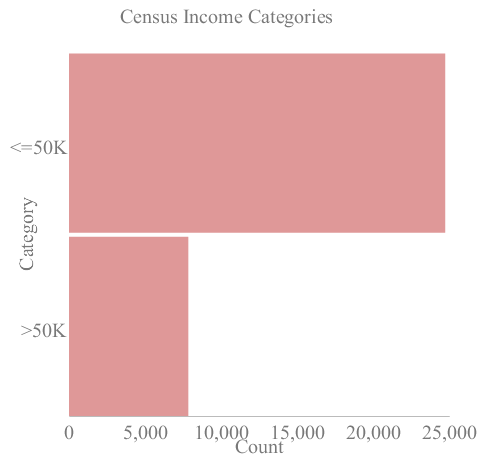
\includegraphics[scale=0.7]{Census_Conditional.png}
	\caption{A bar chart showing census income category proportions}
\end{figure}
%%%%%%%%%%%%%%%%%%

\paragraph{Bar Chart}
As discussed in Chapter 3, a bar chart is the most appropriate chart to be applied in the case of category comparison. We can see immediately when looking at Figure \ref{fig:conditional} that those who make less than \$50,000 are outnumbered by a rate of roughly 3:1 (in fact, the true proportion is 3.15:1). Given the limited input that is provided in the call to the visualizer, we achieve adequate results in the design of the chart. The labeling is clear and well formatted given the provided input. Even without the provision of labels from the method call, someone with an approximately accurate estimate about the outcome would be able to read the chart without labels. Of course, because we cannot know before the  program is run what values to expect, there are some limitations to the way in which we format the results. A good example of this is the x axis. If we desired axis value differences of less or more than 5,000 or a starting point other than 0 it is not a trivial change to make. However, because the purpose of this type of visualization is focused on getting a sense of data in the in-situ context rather than performing detailed visual analysis, it could be argued that such changes are unnecessary.

%%%%%%%%%%%%%%%%%%%%%%%%%%%%%%%%%%%%%%%%%%%%%%%%%%%%%%%%%%%%%%%%%%%%%%%%%%%%
%%%%%%%%%%%%%%%%%%%%%%%%%%%%%%%%%%%%%%%%%%%%%%%%%%%%%%%%%%%%%%%%%%%%%%%%%%%%
\section{Network Analysis}
\label{sec:network}
\INITIAL{N}{etwork data sets are ubiquitous} in many fields, as was briefly discussed in Chapter 3. We will examine some of the basic analyses identified by the KONECT project \cite{Kunegis2013}, and use one of the datasets they have provided in order to enable simple comparison of results and reproduction of visualizations which have been proven useful.

\paragraph{Les Misérables}
Firstly, we will examine a graph representing data extracted from the novel "Les Misérables" by Victor Hugo. Representing only a single work rather than a corpus of texts, this data set is relatively small. This enables us to examine the features of network data in general, and also those visualizations which relate to layout and will only be applicable with sufficiently few nodes. Within this network, each node represents a character in the narrative of the plot, and the edges represent a meeting between two characters. Each edge is weighted with an integer, representing the number of distinct times that the characters appear together. In summary, the graph is undirected and weighted.

%%%%%%%%%%%%%%%%%% 
\begin{figure}
	\centering
	\begin{minipage}{0.45\textwidth}
		\centering
		\label{fig:edgeweightslesmis}
		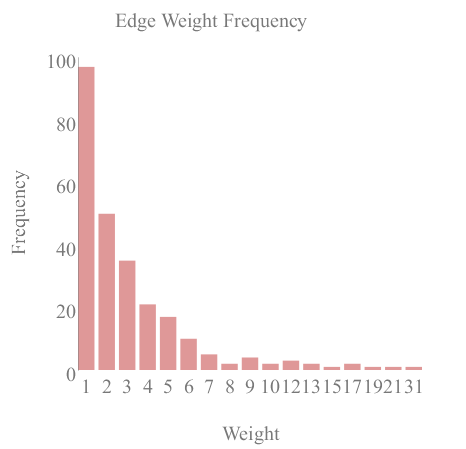
\includegraphics[scale=0.5]{edge_weights_lesmis_inverted.png}
		\caption{A bar chart showing edge weights in the Les Miserables network}
	\end{minipage}\hfill
	\begin{minipage}{0.45\textwidth}
		\centering
		\label{fig:edgeweightskonect}
		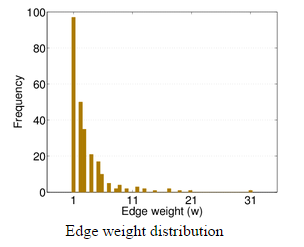
\includegraphics[scale=0.9]{konect_lesmis_edgeweight.png}
		\caption{A bar chart showing edge weights from KONECT}
	\end{minipage}
\end{figure}
%%%%%%%%%%%%%%%%%%

%%%%%%%%%%%%%%%%%% 
\begin{figure}
	\centering
	\begin{minipage}{0.45\textwidth}
		\centering
		\label{fig:edgeweightslesmis}
		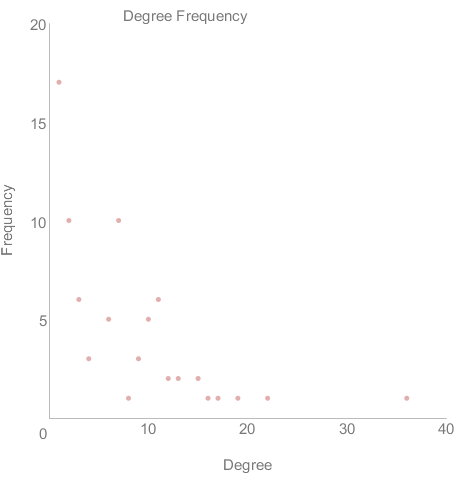
\includegraphics[scale=0.5]{degree_freq_lesmis.png}
		\caption{A scatter plot showing degree frequency in the Les Miserables network}
	\end{minipage}\hfill
	\begin{minipage}{0.45\textwidth}
		\centering
		\label{fig:edgeweightskonect}
		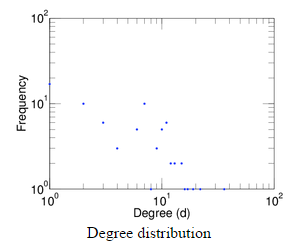
\includegraphics[scale=0.9]{konect_lesmis_degdist.png}
		\caption{A scatter plot showing degree frequency from KONECT}
	\end{minipage}
\end{figure}
%%%%%%%%%%%%%%%%%%